\subsection{Centralization}

One of the major concern with a permissionless blockchain, such as Ethereum,
is the centralization risk. Indeed, if the number of miners and also of full
node diminishes, it is easier that Ethereum would be manipulated by a single
entity.

The risk is concrete, because the requirements to run a full node or 
stand-alone miners are continuously growing. Essentially these nodes should
keep in the storage:
\begin{itemize}
    \item The world-state~\autoref{sec:world-state}
    \item The whole blockchain~\autoref{sec:world-state}
    \item The DAG's cache~\autoref{sec:consensus}
    \item In case the node is a miner, the DAG~\autoref{sec:consensus}
\end{itemize}

\begin{figure*}
    \begin{subfigure}[b]{0.5\textwidth}
        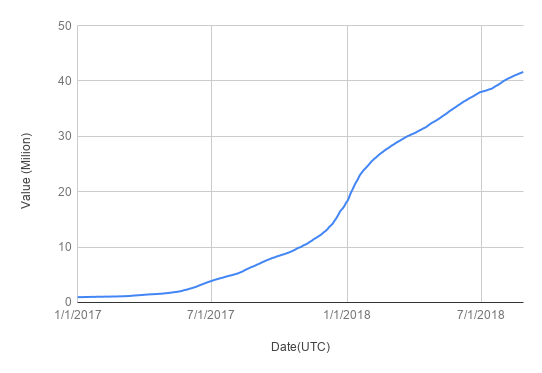
\includegraphics[width=\textwidth]{./res/img/address-growth.png}
        \caption{Unique address growth}
        \label{fig:address-chart}
    \end{subfigure}
    \begin{subfigure}[b]{0.5\textwidth}
        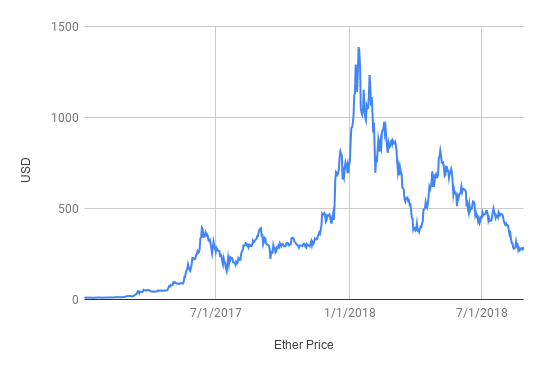
\includegraphics[width=\textwidth]{./res/img/chart_price.png}
        \caption{Ether price evolution}
        \label{fig:price-chart}
    \end{subfigure}
    \begin{subfigure}[b]{0.5\textwidth}
        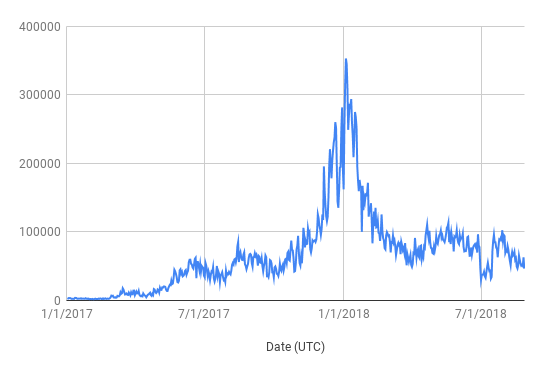
\includegraphics[width=\textwidth]{./res/img/address-growth-rate.png}
        \caption{Address growth rate}
        \label{fig:address-growth-rate-chart}
    \end{subfigure}
    \caption{Ethereum main net charts}
\end{figure*}
The size of the world state is proportional to the number of addresses, because
new addresses require an account state (~\autoref{sec:world-state}. 
\autoref{fig:address-chart} shows the growth in the number of address from the 
beginning of $2017$. We notice that the number of unique address in the 
Ethereum main net has exceeded the $40$ million units and that the growth 
rate~\autoref{fig:address-growth-rate-chart} follows the price evolution of the 
Ether~\autoref{fig:price-chart}, the currency of Ethereum. Indeed, around 
beginning of year $2018$ the growth is no more exponential but rather linear,
because the growth rate is constant.